%Esta seccion trata acerca de conceptos básicos.
\subsection{Java AWT}

AWT (por sus siglas en inglés Abstract Window Toolkit) es una API para 
el desarrollo de aplicaciones en java. \\
Los componentes de AWT son de plataforma dependiente, es decir, que de acuerdo
al sistema operativo es como mostrará cada unos de los componentes con el estilo 
propio, debido a que los componentes usan los recursos que ofrece el sistema 
operativo.\\
La librería java.awt provee paquetes de clases, tales como, Label, TextField, 
TextArea, CheckBox, Choice, List, etc. \\

\subsection{Lista de instrucciones}
\begin{itemize}
	\item \textbf{LINE}: Instrucción para dibujar líneas.
	\item \textbf{CIRCLE}: Instrucción para dibujar círculos.
	\item \textbf{RECTANGLE}: Instrucción para dibujar rectángulos.
	\item \textbf{IMAGE}: Instrucción para dibujar imágenes.
	\item \textbf{COLOR}: Instrucción para colorear contornos.
\end{itemize}

\subsection{Maquina virtual de Pila}
Para la incorporación de nuevas instrucciones en un lenguaje determinado se necesita 
generar código de forma sencilla, de forma estructurada. Por otro lado, también se 
necesita la eliminación de la recursividad ya que en tiempo de procesamiento no es
recomendable hacer uso de una pila de llamadas a función a nuvel sistema operativo. \\
La siguiente figura nos muestra cómo se deben de guardar las instrucciones en una
RAM virtual o una pila en términos de software.

\begin{figure}[H]
	\begin{center}
		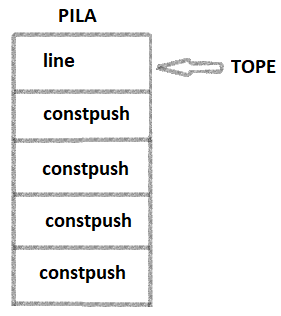
\includegraphics[scale=0.9]{images/img_estr_stack}
		\caption{Estructura para generación de código para la instrucción LINE.}
	\end{center}
\end{figure}